%% SmartLocker, ACM two-column proceedings (sigconf) version for ICIIT 2027 (ACM ICPS), condensed to 5 pages.
%% Condensed from ../smartlocker-acm-10p.tex (single-column, 10 pages): every number is taken from it; the text is
%% shortened and its Table 1 (contributions), Table 4 (simulated channels), Fig. 2 (decision flow) and Fig. 3 (Weka
%% chart) are left out.
%% Build here: tectonic -X compile smartlocker-sigconf.tex
\documentclass[sigconf,screen]{acmart}

\usepackage{booktabs}
\usepackage{array}
\usepackage{textcomp}
\usepackage{adjustbox}
\usepackage{tikz}
\usetikzlibrary{arrows.meta,positioning,fit,shapes.geometric,calc,backgrounds}
\newcommand{\revisioncommit}{fd05eb9}
\setlength{\emergencystretch}{2em}   % long \texttt names in the narrow two-column layout
% no \raggedbottom here: with it, TeX broke columns early before headings and left half of page 3 empty

% Pastel fills, borders and TikZ styles shared with the IEEE version
\definecolor{slBlue}{HTML}{DCEBFA}   % light blue: clients, entry points
\definecolor{slMint}{HTML}{DDF3E3}   % mint green: server, processing
\definecolor{slYellow}{HTML}{FFF3C4} % pale yellow: decisions, services
\definecolor{slPeach}{HTML}{FFE2C8}  % peach: hardware outputs, data access
\definecolor{slCoral}{HTML}{FFD9D6}  % light coral/pink: alerts, outcomes
\definecolor{slSky}{HTML}{E9F6FB}    % very light cyan: group backgrounds
% Dark borders (one per fill) and ink
\definecolor{slBlueD}{HTML}{1F4E79}
\definecolor{slMintD}{HTML}{1E6B3A}
\definecolor{slYellowD}{HTML}{7A5B00}
\definecolor{slPeachD}{HTML}{8A4513}
\definecolor{slCoralD}{HTML}{9B2226}
\definecolor{slInk}{HTML}{0F2338}    % arrows and lines (dark navy)

\tikzset{
  slbox/.style={draw=slBlueD, fill=slBlue, rounded corners=3pt, line width=0.7pt, align=center,
                font=\small, text=black, inner xsep=5pt, inner ysep=4pt, minimum height=0.8cm},
  slblue/.style={slbox},
  slmint/.style={slbox, draw=slMintD, fill=slMint},
  slyellow/.style={slbox, draw=slYellowD, fill=slYellow},
  slpeach/.style={slbox, draw=slPeachD, fill=slPeach},
  slcoral/.style={slbox, draw=slCoralD, fill=slCoral},
  sldec/.style={draw=slYellowD, fill=slYellow, diamond, aspect=2.1, line width=0.7pt, align=center,
                font=\small, text=black, inner sep=1pt},
  slterm/.style={slbox, draw=slCoralD, fill=slCoral, line width=1.0pt},
  slok/.style={slbox, draw=slMintD, fill=slMint, line width=1.0pt},
  slarr/.style={draw=slInk, line width=0.8pt, -{Latex[length=2.4mm, width=1.7mm]}},
  sldbl/.style={draw=slInk, line width=0.8pt, {Latex[length=2.4mm, width=1.7mm]}-{Latex[length=2.4mm, width=1.7mm]}},
  slret/.style={slarr, dashed},
  sllbl/.style={font=\small, text=black, inner sep=2pt},
  slbus/.style={font=\footnotesize, text=slInk, fill=white, inner sep=1.5pt},
  slgroup/.style={draw=slMintD, dashed, rounded corners=5pt, line width=0.7pt},
  slgrouplbl/.style={font=\small\bfseries, text=slMintD, inner sep=2pt},
}
\newcommand{\slsub}[1]{\\[-1pt]{\footnotesize #1}}
\tikzset{every picture/.style={line width=0.6pt}}

%% Rights and conference data: the rights block is filled in from the ACM rights form at camera-ready time.
\setcopyright{none}
\copyrightyear{2027}
\acmYear{2027}
\acmConference[ICIIT 2027]{2027 12th International Conference on Intelligent Information Technology}{March 04--07,
  2027}{Ho Chi Minh City, Vietnam}
\acmBooktitle{2027 12th International Conference on Intelligent Information Technology (ICIIT 2027), March 04--07,
  2027, Ho Chi Minh City, Vietnam}
\acmDOI{}
\acmISBN{}
\renewcommand\footnotetextcopyrightpermission[1]{}   % review copy only: delete this line at camera-ready

\begin{document}

\title{Smart Locker with Anomalous Access Detection Based on IoT Device Telemetry}

\author{Duc Hoang Nguyen}
\authornote{Corresponding author.}
\orcid{0009-0006-9780-8146}
\email{duchoang.nguyen103@gmail.com}
\affiliation{%
  \institution{FPT University}
  \city{Ho Chi Minh City}
  \country{Vietnam}}

\author{Viet Tien Nguyen}
\email{tiennguyen100306@gmail.com}
\affiliation{%
  \institution{FPT University}
  \city{Ho Chi Minh City}
  \country{Vietnam}}

\author{Huy Hoang Nguyen}
\email{huyhoang.ct06@gmail.com}
\affiliation{%
  \institution{FPT University}
  \city{Ho Chi Minh City}
  \country{Vietnam}}

\author{Thanh Cao Nguyen}
\email{thanhcao19112006@gmail.com}
\affiliation{%
  \institution{FPT University}
  \city{Ho Chi Minh City}
  \country{Vietnam}}

\author{Thu Le}
\email{thulvm@fpt.edu.vn}
\affiliation{%
  \institution{FPT University}
  \city{Ho Chi Minh City}
  \country{Vietnam}}

\author{Trong Khanh Kieu}
\email{khanhkt@fpt.edu.vn}
\affiliation{%
  \institution{FPT University}
  \city{Ho Chi Minh City}
  \country{Vietnam}}

\renewcommand{\shortauthors}{D. H. Nguyen et al.}

\begin{abstract}
Campus lockers are still opened with keys or paper codes and cannot be reserved; once networked, their unlock signal
can be forged or replayed. This paper presents SmartLocker, a locker rental system in which users reserve a slot on a web map,
pay from a prepaid wallet and open it with a personal identification number (PIN), a radio-frequency identification
(RFID) card, a fingerprint or a phone page. The ESP32 box takes no access decision: it forwards every credential to the
server, which replies \texttt{UNLOCK} or \texttt{DENY}. Abnormal access (sensor faults, spoofed remote opens, lost
cards, forced opening, wrong-user access, items left behind and overdue storage) is detected mainly by a
priority-ordered rule engine over device telemetry and server context; a machine-learning risk score raises an alert
only for sessions that no rule explains. On synthetic sessions, the best of four Weka classifiers confused mainly wrong-user and
normal sessions, which share the same telemetry by construction, so identity is checked by rule. All automated tests
and replayed scenarios passed, two scenarios after a fix, and server-side processing of every timed device request took
under 40~ms on one laptop. In a simulation through the live device API, a multi-sensor rule prototype outperformed a
partial-parity rule comparator (macro-F1 0.780 against 0.658) but missed most tamper sessions and stayed below learned
classifiers; the simulated distributions are assumed, so these results do not predict field performance.
\end{abstract}

\begin{CCSXML}
<ccs2012>
 <concept>
  <concept_id>10002978.10002997.10002999</concept_id>
  <concept_desc>Security and privacy~Intrusion detection systems</concept_desc>
  <concept_significance>500</concept_significance>
 </concept>
 <concept>
  <concept_id>10010520.10010553</concept_id>
  <concept_desc>Computer systems organization~Embedded and cyber-physical systems</concept_desc>
  <concept_significance>300</concept_significance>
 </concept>
 <concept>
  <concept_id>10010147.10010257</concept_id>
  <concept_desc>Computing methodologies~Machine learning</concept_desc>
  <concept_significance>100</concept_significance>
 </concept>
</ccs2012>
\end{CCSXML}

\ccsdesc[500]{Security and privacy~Intrusion detection systems}
\ccsdesc[300]{Computer systems organization~Embedded and cyber-physical systems}
\ccsdesc[100]{Computing methodologies~Machine learning}

\keywords{Smart locker, Internet of Things, ESP32, RFID, anomaly detection, rule engine, machine learning, Weka}

\maketitle

\section{Introduction}

Self-service lockers are now common for parcels and short-term storage \cite{iwan2016parcel}, but campus lockers
remain mechanical: a slot cannot be booked in advance, and a forced door, a lost key used by someone else or items
left for days are noticed only when reported. Connecting lockers through the Internet of Things (IoT)
\cite{alfuqaha2015iot} makes slot states visible, but a box can then be impersonated, an unlock message forged or
replayed, and sensor readings manipulated \cite{sicari2015security,roman2013features}.

SmartLocker treats the box as a thin, authenticated client and lets the server, which alone holds the booking context,
take every decision. Its contributions are (1) a rental system with map reservation, a prepaid wallet and four
opening methods, in which all money and time rules run in SQL transactions (Sections~\ref{sec:design}
and~\ref{sec:impl}); (2) the main contribution, a priority-ordered rule engine over telemetry and server context with a
hash-chained audit log and a secondary machine-learning (ML) risk score (Section~\ref{sec:detector}); and (3) an
evaluation with automated tests, replayed
scenarios, response times, a classifier comparison on synthetic data and a simulated multi-sensor study
(Section~\ref{sec:ml}).

\section{Related Work}

\textit{Smart and parcel lockers.} Parcel-locker research focuses on last-mile logistics \cite{iwan2016parcel}; a
recent review finds only one sustainability study on safety and security \cite{zhang2025parcel}. An RFID-based IoT locker
\cite{rfidiot2023locker} identifies users by identity card and logs accesses over Wi-Fi; SmartLocker instead checks
every credential in server-side transactions and adds context rules, telemetry scoring and a hash-chained audit log.

\textit{IoT security and anomaly detection.} IoT entities face node capture, eavesdropping and loss of control
\cite{roman2013features} and need authentication and access control beyond traditional countermeasures
\cite{sicari2015security}; RFID credentials can be cloned, replayed and relayed \cite{mitrokotsa2010rfid}. Anomaly
detection techniques include classification-based (also rule-based), nearest-neighbor, clustering and statistical ones
\cite{chandola2009anomaly}; in IoT, learned detectors dominate and scarce labels favor unsupervised ones
\cite{demedeiros2023anomaly}. Like SmartLocker, Shahin et al. \cite{shahin2025twostage} detect in two tiers: a generative model flags
anomalous traffic and a gradient-boosting classifier labels it, with 99.14\% average end-to-end accuracy on N-BaIoT.
Learned intrusion detectors are hard to interpret \cite{sommer2010outside}, and each of 30 machine-learning papers from
top security venues showed at least three of ten pitfalls (P1 to P10) \cite{arp2022dos}. SmartLocker therefore puts
explicit rules first and uses a Weka model \cite{hall2009weka} only as a supporting score; its audit log is
hash-chained \cite{haber1991timestamp} and passwords are hashed with BCrypt \cite{provos1999bcrypt}.

\section{System Design}\label{sec:design}

\subsection{Architecture, Roles and Data}

SmartLocker has three tiers (Fig.~\ref{fig:arch}): web browsers, a phone unlock page and the ESP32 box are the
clients; a Java~8 Servlet/JSP application (MVC2) on Apache Tomcat~9 is the application tier; and SQL Server, which
also implements the business rules as stored procedures, is the data tier. Every outcome is stored as a booking
change, an alert or an audit entry.

\begin{figure*}[tbp]
\centering
\begin{adjustbox}{max width=0.54\textwidth}
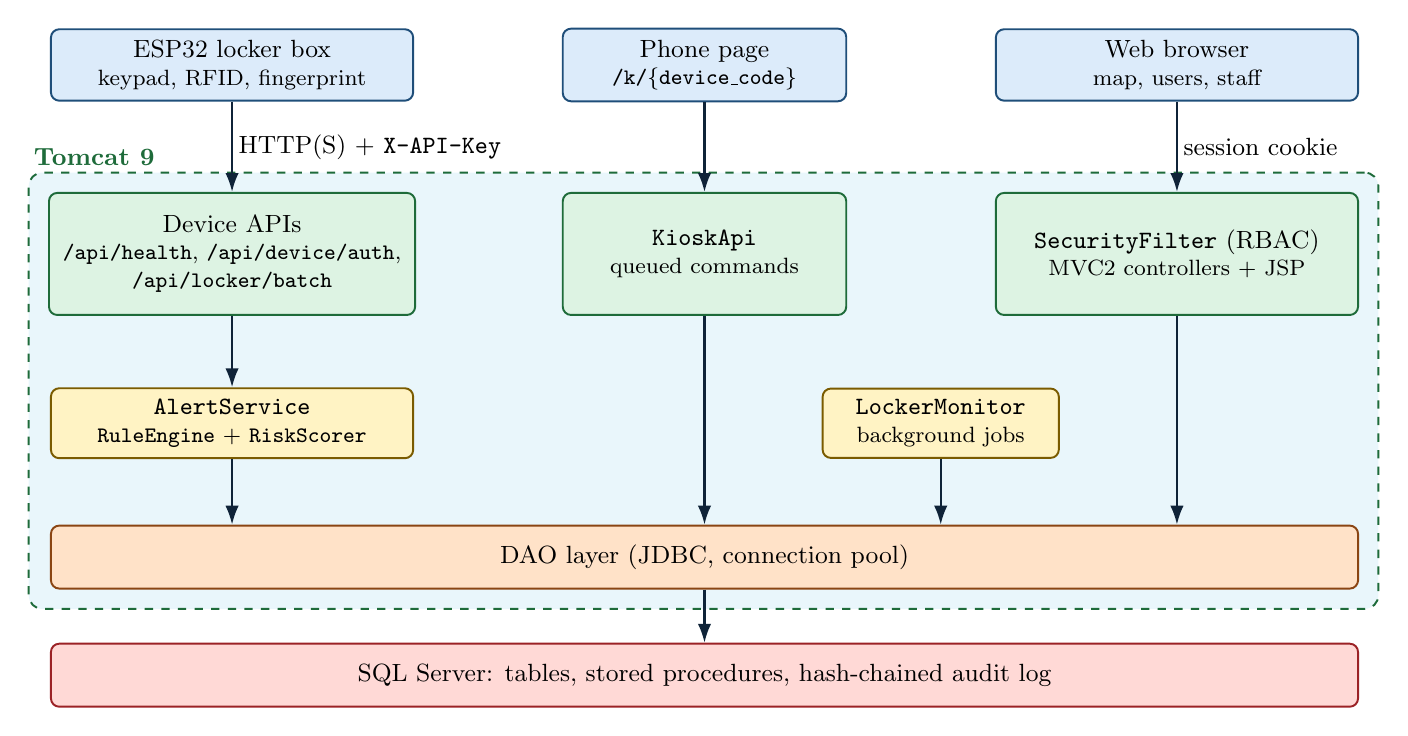
\begin{tikzpicture}
  % clients (top row)
  \node[slblue, minimum width=4.6cm] (esp)   at (2.4,4.3)  {ESP32 locker box\slsub{keypad, RFID, fingerprint}};
  \node[slblue, minimum width=3.6cm] (phone) at (8.4,4.3)  {Phone page\slsub{\texttt{/k/\{device\_code\}}}};
  \node[slblue, minimum width=4.6cm] (web)   at (14.4,4.3) {Web browser\slsub{map, users, staff}};
  % application tier
  \node[slmint, minimum width=4.6cm, minimum height=1.55cm] (devapi) at (2.4,1.9)
       {Device APIs\slsub{\texttt{/api/health}, \texttt{/api/device/auth},}\slsub{\texttt{/api/locker/batch}}};
  \node[slmint, minimum width=3.6cm, minimum height=1.55cm] (kiosk) at (8.4,1.9)
       {\texttt{KioskApi}\slsub{queued commands}};
  \node[slmint, minimum width=4.6cm, minimum height=1.55cm] (ctrl) at (14.4,1.9)
       {\texttt{SecurityFilter} (RBAC)\slsub{MVC2 controllers + JSP}};
  \node[slyellow, minimum width=4.6cm] (svc) at (2.4,-0.25) {\texttt{AlertService}\slsub{\texttt{RuleEngine} + \texttt{RiskScorer}}};
  \node[slyellow, minimum width=3.0cm] (mon) at (11.4,-0.25) {\texttt{LockerMonitor}\slsub{background jobs}};
  \node[slpeach, minimum width=16.6cm] (dao) at (8.4,-1.95) {DAO layer (JDBC, connection pool)};
  % data tier
  \node[slcoral, minimum width=16.6cm] (db) at (8.4,-3.45) {SQL Server: tables, stored procedures, hash-chained audit log};
  % arrows: client to entry point
  \draw[slarr] (esp)   -- node[sllbl, right] {HTTP(S) + \texttt{X-API-Key}} (devapi);
  \draw[slarr] (phone) -- (kiosk);
  \draw[slarr] (web)   -- node[sllbl, right] {session cookie} (ctrl);
  % arrows inside Tomcat
  \draw[slarr] (devapi) -- (svc);
  \draw[slarr] (svc)    -- (svc |- dao.north);
  \draw[slarr] (kiosk)  -- (kiosk |- dao.north);
  \draw[slarr] (mon)    -- (mon |- dao.north);
  \draw[slarr] (ctrl)   -- (ctrl |- dao.north);
  \draw[slarr] (dao)    -- (db);
  \begin{scope}[on background layer]
    \node[slgroup, fill=slSky, fit=(devapi)(kiosk)(ctrl)(svc)(mon)(dao), inner xsep=7pt, inner ysep=7pt,
          label={[slgrouplbl, anchor=south west]north west:Tomcat 9}] (tc) {};
  \end{scope}
\end{tikzpicture}
\end{adjustbox}
\caption{Three-tier architecture of SmartLocker, in which the ESP32 box, the phone page and the web browser reach the
Tomcat application through separate entry points and every outcome is stored in SQL Server.}
\label{fig:arch}
\Description{Block diagram with three clients on top (ESP32 locker box, phone page, web browser), each reaching its own entry point inside Tomcat (device APIs, KioskApi, SecurityFilter with MVC2 controllers), service boxes AlertService and LockerMonitor below, a DAO layer, and SQL Server at the bottom.}
\end{figure*}

Role-based access control defines five roles (end user, operator, technician, auditor and administrator), and all
staff actions are audited. An \emph{area} is a map pin, a \emph{bank} is
a column of lockers controlled by one device, and a \emph{slot} is a 20, 40 or 60~cm cube. Filtered unique indexes
reject a second open booking for the same slot or user, a trigger keeps access sessions append-only, and wallet
deductions run in transactions with exclusive row locks.

\subsection{Hardware}

The box uses an ESP32 board (firmware 4.3) with a 4$\times$4 keypad, a PN532 NFC card reader, an AS608 fingerprint
sensor, a 16$\times$2 I$^2$C LCD, two servos for bolt and door, and an SRF05 ultrasonic sensor; the door locks 20~s
after the person has left, or at the latest 120~s after opening. No door switch, load cell or accelerometer is
fitted and the firmware does not upload access sessions, so door time, weight and inertial readings exist only in the
simulator of Section~\ref{sec:sim_eval}, and no physical validation of door, load or tamper sensing is claimed.

\subsection{Device Protocol and Booking Lifecycle}

Each box holds a secret API key whose SHA-256 hash alone is stored, and the server derives the device identity from
the key, never from the request body. \texttt{POST /api/health} is a 3~s heartbeat that returns pending commands and
blocked card UIDs; \texttt{POST /api/device/auth} submits a PIN, card UID or finger slot and receives
\texttt{UNLOCK}, \texttt{DENY}, \texttt{CHOOSE} (open the slot or check out) or \texttt{CONFIRM\_EMAIL} (the owner
must confirm a card pick-up); and \texttt{POST /api/locker/batch}
uploads access sessions with a sequence number, so a resent session is stored once. A remote or phone open arrives
with the next heartbeat and returns as a session carrying the command id.

A reservation charges the wallet and holds the slot for 15~minutes, after which an unopened booking ends as
\texttt{NO\_SHOW}. An overdue opened booking is never released: after the grace period the slot is locked, each late hour costs 150\% of the hourly rate, and after 48~hours an
\texttt{OVERDUE\_ESCALATED} alert goes to staff.

\section{Anomalous Access Detection}\label{sec:detector}

\subsection{Access Sessions and Context}\label{sec:sessions}

Each door event or rejected card scan produces an \emph{access session} with five features: door time (s), weight
change (g), unlock count, whether a valid local credential was accepted, and stay time (min), plus the opening source,
the card UID and, for a remote or phone open, the command id. Because telemetry does not reveal \emph{who} opened the
slot, the server loads the context: card status and owner, booking owner, whether the remote command was issued and is
unused, allowed stay, valid sensor ranges, calibration validity and the box clock offset.

\subsection{Tier 1: Priority-Ordered Rule Engine}

The rules of Table~\ref{tab:rules} run in a fixed order and the first match sets the label, so faulty readings are
not reported as a break-in and a legitimate remote open not as a forced opening. The valid ranges (door 0 to 3600~s,
weight change $-200$ to 20\,000~g, stay 0 to 10\,080~min) are stored in the database. Rule 2' is the negative branch of
rule 2; column Tests counts the 13 of the 14 rule-engine unit tests that end in a label, and S marks rules also
reached by a replayed scenario (Section~\ref{sec:functional}).

\begin{table*}[tbp]
\centering
\footnotesize
\caption{Detection Rules in Priority Order.}
\label{tab:rules}
\begin{adjustbox}{max width=\textwidth}
\begin{tabular}{c l p{10.6cm} l c}
\toprule
\# & Label & Condition & Action & Tests \\
\midrule
1 & SENSOR\_FAULT & door time, weight change or stay time outside valid range; door open longer than stay; box clock over 300~s ahead; weight calibration expired & Alert, ticket, no ML & 3, S \\[2pt]
2 & STAFF\_OPEN & remote or phone open with a valid, unused command for this slot, issued at most 30~min before the session (box clock up to 60~s behind tolerated) & Command done, no alert & 2, S \\[2pt]
2' & SUSPECTED\_SPOOF & remote or phone open without a valid, unused command & Alert & 1, S \\[2pt]
3 & LOST\_CARD\_USED & the presented card is not active (reported lost or blocked) & Alert & 1, S \\[2pt]
4 & FORCED\_OPEN & the door opened locally without an accepted PIN, active card or fingerprint & Alert & 1 \\[2pt]
5 & WRONG\_USER & an active card whose owner is not the owner of the slot booking & Alert & 1 \\[2pt]
6 & SUSPECTED\_SPOOF & the weight changed by more than 50~g while the door time stayed at 0~s (unreported open) & Alert & 1 \\[2pt]
7 & ITEM\_LEFT & the weight change is above $+50$~g (read as items left after pick-up) & Alert & 1 \\[2pt]
8 & OVERDUE & stay time longer than the plan allows & Alert & 1 \\[2pt]
9 & NORMAL & no rule matched & Tier 2 & 1 \\
\bottomrule
\end{tabular}
\end{adjustbox}
\end{table*}

\subsection{Tier 2: Machine-Learning Risk Score}

Let $\mathbf{x}_s = (d, w, u, v, t)$ denote the five features of a session $s$. A classifier trained offline on
labeled sessions estimates the probability that $s$ is normal, and the \emph{risk score} is
\begin{equation}
r(s) = 1 - P\left(y = \text{NORMAL} \mid \mathbf{x}_s\right).
\label{eq:risk}
\end{equation}
The deployed model is the six-class classifier with the highest weighted F1, currently IBk ($k=5$). With $\ell(s)$ the
label of the first rule of Table~\ref{tab:rules} that matches $s$ and $\mathcal{L}_0 = \{\text{NORMAL},
\text{STAFF\_OPEN}\}$ the labels that raise no alert, the alert raised for $s$ is
\begin{equation}
A(s) =
\begin{cases}
\ell(s), & \ell(s) \notin \mathcal{L}_0,\\
\text{ML\_ANOMALY}, & \ell(s) = \text{NORMAL} \text{ and } r(s) \geq \tau,\\
\text{none}, & \text{otherwise},
\end{cases}
\label{eq:alert}
\end{equation}
with $\tau = 0.80$, so at least four of the five nearest neighbors must be abnormal. When a rule matches, $r(s)$ is
stored with its alert as evidence; it is never computed for SENSOR\_FAULT or STAFF\_OPEN. A STAFF\_OPEN marks its
command done through a conditional update, so of two sessions carrying one command only one is a staff open and the
other is SUSPECTED\_SPOOF; a SENSOR\_FAULT takes the slot out of service and opens a ticket.

\subsection{Server-Side Safeguards and Audit Log}\label{sec:safeguards}

Five wrong PINs, cards or fingers within 5~minutes lock the box for 120~s; a job running every 15~s marks a box
silent for 90~s as \texttt{OFFLINE} with a \texttt{DEVICE\_OFFLINE} alert; a card reported lost is pushed to the box
with the next heartbeat; and a valid card at the wrong box is logged as \texttt{WRONG\_PLACE}. Every business action
and alert is appended to an audit log whose entries store the SHA-256 hash of their fields and of the previous entry
\cite{haber1991timestamp}. The last entry is read under an update lock, so concurrent writers cannot fork the chain;
altering, deleting, inserting or reordering an entry inside the chain breaks the next link, and a job re-verifies the
chain every 60~s. Without an external anchor the chain cannot reveal changes at its tail or an administrator who recomputes every
hash, so it is tamper-evident rather than a full time-stamping protocol.

\section{Implementation}\label{sec:impl}

The server has about 11\,800 lines of Java~8 (with comments and blank lines) in 89 files and 22 JSP views, and uses
Gson, jBCrypt
\cite{provos1999bcrypt} and Weka \cite{hall2009weka}. Every money or time rule is a stored procedure
that locks its rows with \texttt{UPDLOCK, HOLDLOCK}, so a slot cannot be booked or an extension charged twice. All user
input goes through JDBC prepared statements and is escaped in JSP and JavaScript, and every state-changing request
except sign-up and sign-in needs a permitted user, the phone-page PIN or a single-use e-mail token.

\section{Evaluation}\label{sec:ml}

\subsection{Experimental Setup}

\textit{Dataset.} The risk model is trained on 480 synthetic rows of the five features from the seed script
\texttt{sql/02\_data\_v1.sql}, 80 in each class (NORMAL, FORCED\_OPEN, WRONG\_USER, OVERDUE, ITEM\_LEFT and
SUSPECTED\_SPOOF), since no public dataset records the door time, weight change and card of a locker session. The
rows follow simple class patterns on a deterministic grid, and wrong-user rows use the formulas of normal rows.

\textit{Protocol.} Random Forest \cite{breiman2001rf}, J48 \cite{quinlan1993c45}, Naive Bayes \cite{john1995nb} and
IBk \cite{aha1991ibl} were compared with Weka defaults, except $k=5$ for IBk, by stratified 10-fold cross-validation
\cite{kohavi1995cv} (seed 42) on six classes and on NORMAL versus ABNORMAL. All runs used one laptop (Intel Core
i5-11400H, 16~GB RAM, Windows~11; JDK 1.8.0\_202, Weka 3.8.6, Tomcat 9.0.113, SQL Server 2022). Tests and measurements
ran on 17 November 2026 on commit \texttt{\revisioncommit}, to which the code counts also refer; its server, TestNG and
SQL code is unchanged in the final commit. The Weka metrics equal those of a 30 October 2026 run, and the simulation
ran on 16 November 2026 (UTC) on the same code.

\subsection{Classification Results}

IBk achieves the highest weighted F1 on both tasks (Table~\ref{tab:ml}), followed by Random Forest, while Naive Bayes
is weakest on six classes. IBk classifies all FORCED\_OPEN, OVERDUE and SUSPECTED\_SPOOF and 79 of 80 ITEM\_LEFT
sessions correctly; 10 of its 11 errors are wrong-user sessions labeled normal (7) or the reverse (3), and Random
Forest errs the same way (17 and 8). A valid card of another person produces the telemetry of a normal visit, and
without the WRONG\_USER rows IBk misclassifies only 1 of 400 sessions. Wrong-user access is therefore answered by
rule~5, ML alerts are shown to staff as model detections rather than rule matches, and the score should be trusted
only after retraining on real sessions.

\begin{table}[tbp]
\centering
\small
\caption{Offline Weka Study on the 480-Row Dataset (Weighted Averages, Stratified 10-Fold Cross-Validation).}
\label{tab:ml}
\begin{adjustbox}{max width=\columnwidth}
\begin{tabular}{l c c c c c c}
\toprule
 & \multicolumn{4}{c}{Six classes / Multi-class} & \multicolumn{2}{c}{Binary / Detection} \\
Model & Accuracy & Precision & Recall & F1 & Accuracy & F1 \\
\midrule
Random Forest & 0.948 & 0.949 & 0.948 & 0.948 & 0.938 & 0.939 \\
J48 (C4.5)    & 0.856 & 0.857 & 0.856 & 0.856 & 0.831 & 0.848 \\
Naive Bayes   & 0.779 & 0.778 & 0.779 & 0.778 & 0.833 & 0.852 \\
IBk ($k=5$)   & 0.977 & 0.978 & 0.977 & 0.977 & 0.975 & 0.975 \\
\bottomrule
\end{tabular}
\end{adjustbox}
\end{table}

\subsection{Functional Testing}\label{sec:functional}

\textit{Tests.} The TestNG suite has 83 test methods in 14 classes (47 in memory, 36 against database procedures and
HTTP endpoints), including 14 rule-engine tests; all passed. Nineteen Postman/newman scenarios, from
the four opening methods to lockout, no-show, overdue and escalation, ran 241 requests and 514 assertions without a
failure.

\textit{Audit chain.} A read-only export of the simulation audit chain (1\,343 entries) was altered in seven ways,
20 times each (seed 20261116). Modifying, deleting, inserting and swapping inner entries were each detected in 20 of
20 cases, and appending, truncating the tail and a privileged rewrite of every hash each in 0 of 20, as expected
without an anchor; copying the chain head outside the database every ten entries caught 20 of 20 rewrites and 18 of 20
truncations, but no appends (deterministic tests, not detection rates).

\textit{Concurrency and scenarios.} When 50 users reserved one free slot at once and one user reserved 20 slots at
once, exactly one call won each race and only the two winners were charged. A device simulator replayed six scenarios
with the key of the real box LOCKER-01: a silent box became \texttt{OFFLINE} after 99.5~s (expected 90 to 105~s); a
staff remote open became STAFF\_OPEN and its replay SUSPECTED\_SPOOF; an unissued command id gave SUSPECTED\_SPOOF; a
lost card raised LOST\_CARD\_USED; a reservation and its PIN gave \texttt{UNLOCK} and \texttt{CHECK\_IN}; and a
$-5000$~g weight change raised SENSOR\_FAULT. All six gave the expected label, two only after a fix: the remote-open
rule had no clock tolerance and now accepts a session stamped up to 60~s before its command, and the check-in scenario
now sends the PIN to \texttt{/api/device/auth}, as the real box does.

\subsection{Multi-Sensor Simulation}\label{sec:sim_eval}

Channels the box lacks were exercised by a multi-sensor simulation in Python. The generator first fixes a latent
action and its label and then draws noisy observations, so no label depends on a detector; it produced 100 sessions,
20 in each of five categories (normal, unauthorized credential, forced door, load or tamper, and sensor or network
fault), and its version~2 was frozen by hash before any detector ran. Door time, weight, vibration, shock, tilt,
ultrasonic distance and stay are drawn from assumed log-normal, normal or uniform distributions; only network latency
is resampled from 100 measured round trips of \texttt{/api/locker/batch} (2.0 to 39.5~ms). On 16 November 2026 (run
\texttt{RUN\_20261116\_171508\_SEED42\_V2}) a harness sent every credential and session to the device API of the local
stack: every expected \texttt{UNLOCK} or \texttt{DENY} was returned, all 100 sessions were stored, replayed sequence
numbers were rejected, and 99 sessions matched their expected transport outcome (one injected timeout lasted only
3.27~s, below the 5~s limit); the verdicts of the production Java path were then read back. \emph{B0} is a comparator
in partial parity with the production rules: it re-implements the range, lost-card, forced-open and closed-door weight
rules and the credential result; \emph{B1-P} is a prototype that adds hand-set thresholds on ultrasonic distance,
vibration, tilt, shock and network latency. When the Java verdicts are mapped to the five categories, ITEM\_LEFT and
ML\_ANOMALY count as errors.

\begin{table}[tbp]
\centering
\footnotesize
\caption{Detectors on the 100-Session Simulation (Generator Version~2).}
\label{tab:b0_vs_b1}
\setlength{\tabcolsep}{4pt}
\begin{adjustbox}{max width=\columnwidth}
\begin{tabular}{l c c c c}
\toprule
Detector & Macro-F1 & Tamper R. & Fault R. & Macro-F1, 5 seeds \\
\midrule
B0 comparator & 0.658 & 0.150 & 0.500 & $0.610\pm0.038$ \\
B1-P prototype & 0.780 & 0.250 & 0.950 & $0.753\pm0.036$ \\
Java, rules only & 0.616 & 0.150 & 0.500 & live run only \\
Java, rules + risk score & 0.475 & 0.150 & 0.500 & live run only \\
J48, all inputs & 0.980 & 1.000 & 1.000 & $0.980\pm0.010$ \\
Logistic regression & 1.000 & 1.000 & 1.000 & $0.990\pm0.014$ \\
J48, credential + network & 0.546 & 0.000 & 0.250 & $0.537\pm0.022$ \\
\bottomrule
\end{tabular}
\end{adjustbox}
\\[2pt]
\parbox{0.97\linewidth}{\footnotesize Recall (R.) and macro-F1 on the live seed-42 run; 5 seeds (42, 101, 202, 303,
404): mean $\pm$ sample SD; seeds other than 42 were run offline with the expected credential outcome, which the
backend returned for all 100 live sessions.}
\end{table}

B1-P reached a macro-F1 of 0.780 against 0.658 for B0 (Table~\ref{tab:b0_vs_b1}), mostly on faults, whose ultrasonic,
inertial and network symptoms B0 does not see, while both miss most tamper sessions (B1-P labels 15 of the 20 as
normal). For anomaly versus normal, McNemar's test counts 6 sessions that only B1-P gets right and none that only B0
gets right (exact $p=0.031$), and a stratified paired bootstrap (10\,000 resamples) gives $\Delta$macro-F1 $=0.122$
with a 95\% interval of $[0.062, 0.190]$. The production rules alone reach 0.616 but flag 11 of the 20 normal sessions:
8 deposits as ITEM\_LEFT, because rule~7 reads every weight gain above 50~g as items left after pick-up, and 3 pick-ups
of 233 to 943~g as SENSOR\_FAULT, because rule~1 checks the weight range against the weight change; with the risk
score, 31 sessions receive a class-less ML\_ANOMALY alert, so macro-F1 falls to 0.475 while anomaly-versus-normal F1
rises from 0.770 to 0.870, level with B1-P (0.871). J48 trained on the other four seeds with all 12 observable inputs
(sensor, credential, latency and replay fields) reaches 0.980 and is right on 19 sessions where B1-P is wrong,
against 2 the other way ($p=2.2\times10^{-4}$); logistic regression reaches 1.000 (19 against 0), whereas J48 given
only the credential and network fields reaches 0.546, so the labels do not leak through the context. Retrained without
one feature group, J48 gives five-seed means of 0.777 without door and load, 0.881 without the credential context and
at least 0.956 without the network, inertial or ultrasonic group. Scaling the six medians that separate the anomaly
classes (two vibration medians, shock, tilt, forced door time and spoof weight) by 0.7 or 1.3, one at a time
(12 variants) or all together (2), kept B1-P above B0 by 0.12 to 0.16 and below J48 by 0.21 to 0.26 in all 15 runs
including the baseline.

\subsection{Server-Side Response Time}\label{sec:latency}

Only server processing of the device API was timed: 30 curl requests per endpoint from the same laptop after one
warm-up, excluding Wi-Fi, credential reading and servo movement. The median was 7.6~ms for the heartbeat, 16.0~ms for a
PIN at the box and 15.9~ms on the phone page, and no request took longer than 38.6~ms; a phone-page open also waits for
the next heartbeat. The fifth wrong PIN started a 120~s lock that also refused the valid PIN, which was accepted again
120.9~s after the lock started.

\subsection{Threats to Validity and Limitations}\label{sec:limits}

\textit{Internal validity.} Both datasets are synthetic: the Weka rows form a deterministic grid and almost every
simulation distribution is assumed, so the separability J48 exploits reflects these assumptions (sampling bias, P1
\cite{arp2022dos}). The second generator was designed by authors who knew the B1-P thresholds, and three of its
parameters (the forced-door vibration median, the shock clip and the timeout delay) lie within $\pm$20\% of a B1-P
threshold, so data snooping (P3) cannot be ruled out. B0 has partial parity and a learned
tree outperforms B1-P (inappropriate baseline, P6); latent-action labels, a frozen generator, learned baselines, an
ablation, a sensitivity analysis and five seeds mitigate these risks.

\textit{External validity.} All results come from one laptop and one box with a single servo-locked slot; door
switch, load cell and accelerometer are simulated and no campus trace exists (lab-only evaluation, P9). Rules 1 and 7
treat every session as the pick-up of a light item: a deposit of more than 50~g raises ITEM\_LEFT and a pick-up of
more than 200~g raises SENSOR\_FAULT, so both should use the absolute load and the booking phase once a load cell is
fitted. Remaining security risks include the lack of mutual TLS and CSRF tokens, plain HTTP to Tomcat, unanchored audit rewrites and cloned cards
that work until reported. Seeds, code, logs and scripts are available at
\url{https://github.com/HoangDuc1003/SmartLocker}.

\section{Conclusion}

SmartLocker leaves every access decision of its ESP32 box to the server and labels each access session with a
priority-ordered rule tier backed by a tamper-evident audit log; every replayed scenario gave the expected label, two
after a fix. Telemetry alone could not separate wrong-user from normal access, so identity is checked by rule. In
simulation, a multi-sensor rule prototype beat a partial-parity comparator (macro-F1 0.780 against 0.658) but found
only 5 of 20 tamper sessions and stayed below a learned tree (0.980) and logistic regression (1.000). Future work will
fit door, load and inertial sensors, base the weight rules on the absolute load, collect labeled campus sessions,
integrate the audit anchor, and add mutual TLS and CSRF tokens.

\begin{acks}
The authors thank FPT University and the instructors. AI tools (Claude, Anthropic) assisted with English editing,
figures and parts of the simulation and evaluation code; the authors reviewed all such material and take full
responsibility for this paper.
\end{acks}

\bibliographystyle{ACM-Reference-Format}
\bibliography{../smartlocker-acm}

\end{document}
